\documentclass{article}
\usepackage{hyperref}
\usepackage{xcolor}
\usepackage{enumitem}
\usepackage{geometry}
\usepackage{parskip}
\usepackage{graphicx}
\usepackage{tikz}
\usepackage{titlesec}
\usepackage{tcolorbox}
\usepackage{fancyhdr}
\usetikzlibrary{mindmap,trees}

\definecolor{feugreen}{HTML}{1C5310}
\definecolor{feuyellow}{HTML}{FDB813}
\definecolor{feulightgreen}{HTML}{2E7D32}
\definecolor{feugold}{HTML}{FFD700}

\geometry{
    a4paper,
    top=2.5cm,
    bottom=2.5cm,
    left=2.5cm,
    right=2.5cm,
    headheight=21pt
}

\pagestyle{fancy}
\fancyhf{}
\fancyhead[L]{\color{feugreen}GED0085 - Gender and Society}
\fancyhead[R]{\color{feugreen}Far Eastern University}
\fancyfoot[C]{\color{feugreen}\thepage}
\renewcommand{\headrulewidth}{1pt}
\renewcommand{\headrule}{\hbox to\headwidth{\color{feugreen}\leaders\hrule height \headrulewidth\hfill}}

\titleformat{\section}
{\color{feugreen}\Large\bfseries}
{\thesection}{1em}{}[\titlerule]

\titleformat{\subsection}
{\color{feulightgreen}\large\bfseries}
{\thesubsection}{1em}{}

\newtcolorbox{feubox}{
    colback=feugreen!5,
    colframe=feugreen,
    boxrule=0.5pt,
    arc=4pt,
    boxsep=5pt,
    left=6pt,
    right=6pt,
    top=6pt,
    bottom=6pt
}

\tikzset{
    level 1/.style={
        level distance=3.5cm,
        sibling distance=3.5cm,
        concept color=feugreen!40
    },
    level 2/.style={
        level distance=3cm,
        sibling distance=2cm,
        concept color=feuyellow!40
    },
    every node/.style={align=center}
}

\title{
    \includegraphics[width=0.6\textwidth]{FEU-with-Roman.png}\\[1cm]
    {\color{feugreen}\Huge\textbf{GED0085 Website Structure:}}\\[0.5cm]
    {\color{feulightgreen}\Large\textbf{Advocating for Gender Equality}}
}
\author{
    {\Large Far Eastern University Institute of Technology}
}
\date{
    \vspace{1cm}
    {\color{feugreen}\textbf{GENDER AND SOCIETY}}\\[0.3cm]
    {\color{feulightgreen}\textbf{FINAL EXAMINATION}}\\[0.3cm]
    {\color{feugreen}\textbf{Designing and Presenting Gender Advocacy Campaign Plan/Proposal}}
}

% Fix for enumitem negative labelwidth warning
\setlist[description]{
    font=\normalfont,
    style=multiline,
    leftmargin=3em,
    labelindent=0pt,
    labelwidth=2em,
    labelsep=1em,
    align=left
}

\begin{document}

\maketitle

\section*{Introduction}
We are students from Far Eastern University Institute of Technology, driven to promote gender equality as part of the final requirement for our course, Gender and Society (GED0085). Our advocacy is rooted in the values and lessons we've gained from exploring gender as a social construct and analyzing issues of inequality, discrimination, and identity. Through this platform, we aim to raise awareness, inspire change, and create a more inclusive society where everyone, regardless of gender, can thrive.

\section*{Website Sitemap}
\begin{center}
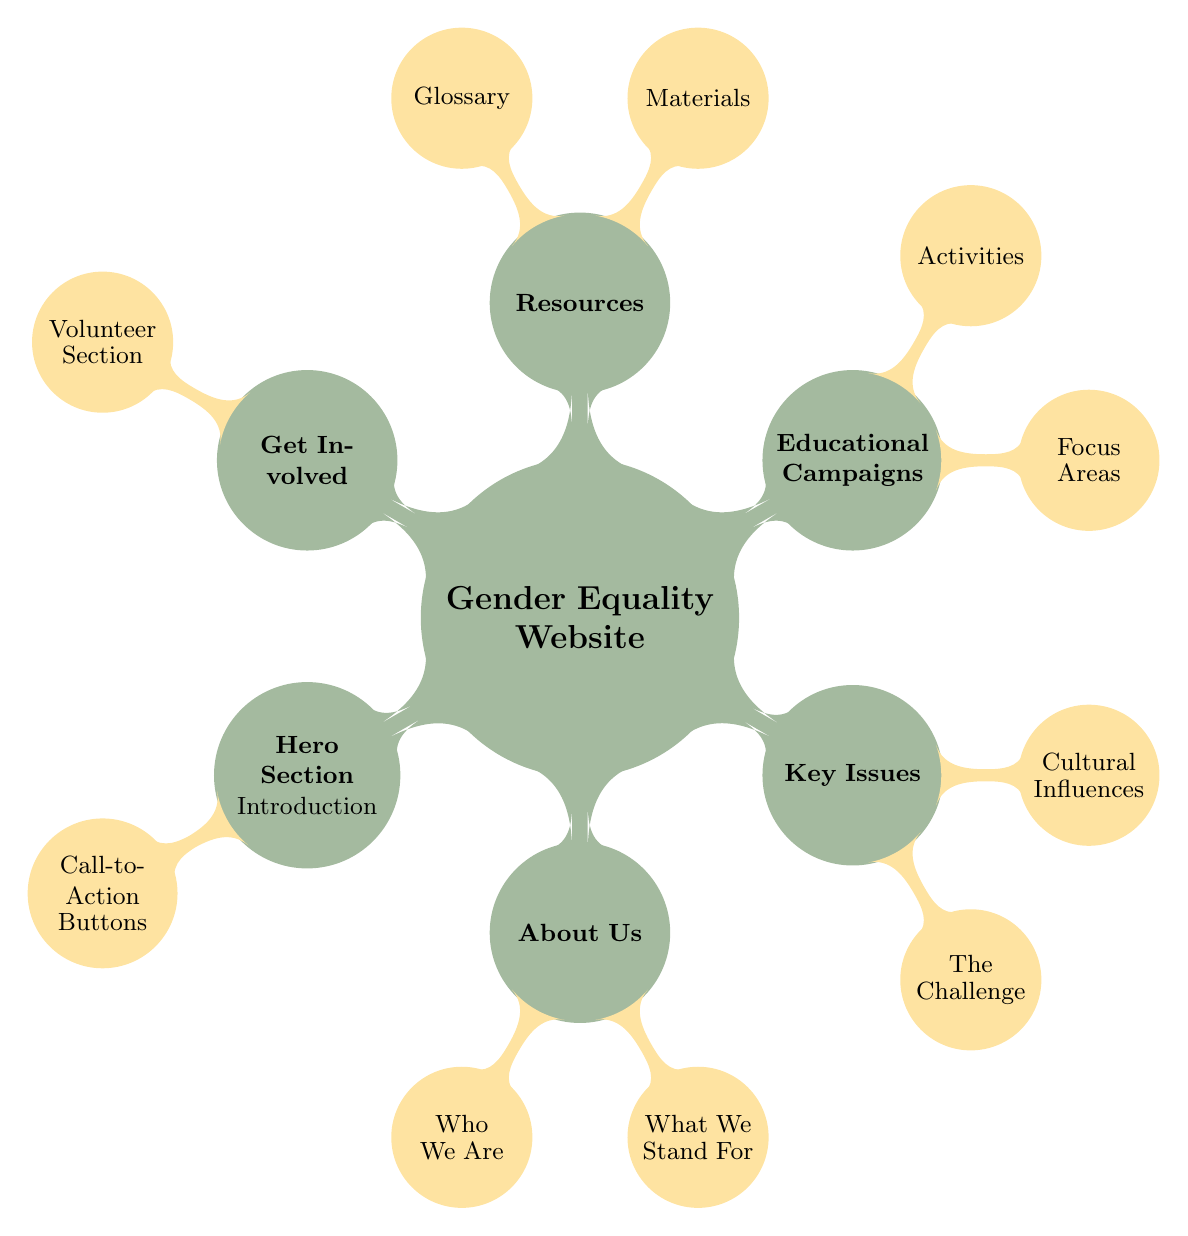
\begin{tikzpicture}[mindmap, grow cyclic, every node/.style=concept, concept color=feugreen!40,
    level 1/.append style={level distance=4cm,sibling angle=60},
    level 2/.append style={level distance=3cm}]

\node{\textbf{Gender Equality\\Website}}
    child { node {\textbf{Hero Section}\\\small{Introduction}}
        child { node {\small{Call-to-Action\\Buttons}} }
    }
    child { node {\textbf{About Us}}
        child { node {\small{Who We Are}} }
        child { node {\small{What We\\Stand For}} }
    }
    child { node {\textbf{Key Issues}}
        child { node {\small{The Challenge}} }
        child { node {\small{Cultural\\Influences}} }
    }
    child { node {\textbf{Educational\\Campaigns}}
        child { node {\small{Focus Areas}} }
        child { node {\small{Activities}} }
    }
    child { node {\textbf{Resources}}
        child { node {\small{Materials}} }
        child { node {\small{Glossary}} }
    }
    child { node {\textbf{Get Involved}}
        child { node {\small{Volunteer\\Section}} }
    };
\end{tikzpicture}
\end{center}

\section*{Purpose of the Campaign}
\subsection*{Our Mission}
To challenge outdated perceptions of gender, promote equality, and celebrate diversity.

\subsection*{Our Goals}
\begin{itemize}[leftmargin=*]
    \item \textbf{Raise Awareness:} Educate our community about the realities of gender inequalities and the significance of inclusivity.
    \item \textbf{Encourage Action:} Inspire individuals to take steps toward building a fair and just society.
    \item \textbf{Foster Engagement:} Provide resources and opportunities for people to actively participate in promoting gender equality.
\end{itemize}

\section*{Website Structure}
\subsection*{1. Hero Section (Introduction)}
\begin{description}
    \item[\textbf{Headline:}] 
    Breaking Barriers, Building Equality: Join the Movement for Gender Justice
    \item[\textbf{Subheadline:}] 
    A project by FEU Tech students for GED0085 - Gender and Society
    \item[\textbf{Call-to-Action Buttons:}]
    \begin{itemize}[label={--}]
        \item Learn More About Gender Equality
        \item Join Our Advocacy Today
    \end{itemize}
\end{description}

\subsection*{2. About Us}
\textbf{Who We Are:} \\
Students passionate about creating a gender-sensitive community by applying the insights and theories learned in Gender and Society (GED0085). \\
\textbf{What We Stand For:} \\
Promoting equality across the gender spectrum by addressing discrimination, advocating for LGBTQIA+ rights, and celebrating diversity.

\subsection*{3. Key Issues}
\textbf{Title:} "Why Gender Equality Matters" \\
\textbf{Content:}
\begin{itemize}
    \item \textbf{The Challenge:} Highlight systemic issues such as wage gaps, underrepresentation, and discrimination.
    \item \textbf{Cultural Influences:} Explain how media, politics, and social norms shape gender perceptions.
    \item Include relevant statistics and examples to emphasize urgency.
\end{itemize}

\subsection*{4. Educational Campaigns}
\textbf{Content:}
\begin{itemize}
    \item \textbf{Our Focus Areas:}
    \begin{itemize}
        \item Gender Sensitivity in Schools
        \item Workplace Inclusion
        \item LGBTQIA+ Advocacy
    \end{itemize}
    \item Use engaging formats such as infographics or videos to explain each initiative.
    \item Provide a schedule of activities or milestones for the project.
\end{itemize}

\subsection*{5. Resources}
\textbf{Content:}
\begin{itemize}
    \item Accessible, student-friendly resources for learning about gender equality.
    \item Downloadable materials: Articles, infographics, and a list of recommended readings or links.
    \item A glossary explaining key terms like "gender spectrum," "social construct," and "intersectionality."
\end{itemize}

\subsection*{6. Get Involved}
\textbf{Volunteer Section:}
\begin{itemize}
    \item \textbf{Headline:} "Help Us Create a Gender-Inclusive Future"
    \item \textbf{Subheadline:} "Join the advocacy of FEU Tech students for GED0085."
    \item Volunteer sign-up form for participation in campaigns or workshops.
\end{itemize}

\section*{Design and Technical Guidelines}
\subsection*{Visual Identity}
\begin{itemize}[leftmargin=*]
    \item \textbf{Colors:} Reflect FEU's spirit with {\color{feugreen}\textbf{GREEN}} for growth and inclusivity and {\color{feuyellow}\textbf{YELLOW}} for optimism and energy.
    \item \textbf{Imagery:} Use high-quality visuals featuring diverse individuals in inclusive settings.
\end{itemize}

\subsection*{Layout}
\begin{itemize}
    \item Dynamic single-page design with smooth navigation between sections.
\end{itemize}

\subsection*{Framework}
\begin{itemize}
    \item Built using Next.js 14 for performance and scalability.
\end{itemize}

\subsection*{Accessibility}
\begin{itemize}
    \item Ensure responsive design, alt text for images, and clear navigation for all users.
\end{itemize}

\section*{Inspiration from the Course}
This project embodies the principles of GED0085 - Gender and Society, applying our understanding of how media, culture, politics, and socioeconomic influences shape gender identity and perception. With this website, we hope to inspire others to adopt a gender-sensitive mindset and actively contribute to equality.

\section*{Evaluation Criteria}
\begin{feubox}
\begin{itemize}[leftmargin=*]
    \item \textbf{Collaboration (20\%)}
    \begin{itemize}
        \item Active participation in group discussions
        \item Equal distribution of tasks
        \item Effective team communication
    \end{itemize}
    
    \item \textbf{Feasibility/Practicality (25\%)}
    \begin{itemize}
        \item Realistic implementation plan
        \item Efficient use of available resources
        \item Clear and achievable objectives
    \end{itemize}
    
    \item \textbf{Class Presentation (35\%)}
    \begin{itemize}
        \item Clear and persuasive delivery
        \item Professional presentation materials
        \item Comprehensive campaign details
    \end{itemize}
    
    \item \textbf{Effectivity (20\%)}
    \begin{itemize}
        \item Impact on target audience
        \item Sustainability of the campaign
        \item Measurable outcomes
    \end{itemize}
\end{itemize}
\end{feubox}

\end{document}